\documentclass[vipdfmx,a4paper,11pt]{jsarticle}
\usepackage{hyperref} % ハイパーリンク差し込み用
\usepackage{pxjahyper} % 目次の文字化け対策

\usepackage[dvipdfmx]{graphicx,xcolor}% ドライバ指定のため

%オートマトン
\usepackage{tikz}
\usetikzlibrary{automata,positioning}
\usetikzlibrary{calc}
\usetikzlibrary{decorations.pathreplacing}
\usetikzlibrary{matrix,backgrounds,fit,positioning}

% 数式
\usepackage{amsmath,amsfonts}
\usepackage{amssymb}
\usepackage{bm}
\usepackage{braket}
\usepackage{multicol}

% 画像
\usepackage[dvipdfmx]{graphicx}

% SI単位
\usepackage{siunitx}

%プログラムリスト用
\usepackage{listings,jvlisting}
\lstset{
basicstyle={\ttfamily},
identifierstyle={\small},
commentstyle={\smallitshape},
keywordstyle={\small\bfseries},
ndkeywordstyle={\small},
stringstyle={\small\ttfamily},
frame={tb},
breaklines=true,
columns=[l]{fullflexible},
numbers=left,
xrightmargin=0zw,
xleftmargin=3zw,
numberstyle={\scriptsize},
stepnumber=1,
numbersep=1zw,
lineskip=-0.5ex
}

\usepackage{tcolorbox}
\newtcbox{\code}[1][]{
  colback=gray!10!white,
  colframe=gray!20!white,
  boxrule=1pt,
  left=0mm,right=0mm,top=0mm,bottom=0mm,
  box align=base,
  nobeforeafter,
  fontupper=\ttfamily
}

\renewcommand{\thesubsection}{\arabic{section}-\arabic{subsection}}
\renewcommand{\thesubsubsection}{\arabic{section}-\arabic{subsection}.\arabic{subsubsection}}
\makeatletter
  \renewcommand{\theequation}{\arabic{subsection}.\arabic{equation}}
  \@addtoreset{equation}{subsection}
\makeatother
\makeatletter
% sectionの下マージンを小さく
\renewcommand{\section}{%
  \@startsection{section}{1}{\z@}%
  {0.4\Cvs}{0.1\Cvs}%
  {\normalfont\large\headfont\raggedright}}
\renewcommand{\subsection}{%
  \@startsection{subsection}{1}{\z@}%
  {0.4\Cvs}{0.1\Cvs}%
  {\normalfont\large\headfont\raggedright}}
\renewcommand{\subsubsection}{%
  \@startsection{subsubsection}{1}{\z@}%
  {0.4\Cvs}{0.1\Cvs}%
  {\normalfont\large\headfont\raggedright}}
\makeatother

\begin{document}

\title{MMCSS tutorial(jp)}
\author{Takanori Saiki}
\date{last update : \today}
\maketitle

\newpage

\section{Introduction}
MMCSS (Multicellular Molecular Communication System Simulator) is a general-purpose simulator for simulating multicellular molecular communication systems. Since the basic program for the simulation is provided, users can easily implement their own simulation models by changing parameters or extending their own simulation models.

\section{Preparation}
This section describes the procedure for installing MMCSS. The environment used is assumed to be Mac OS or Linux,
However, it is also possible to run MMCSS on Windows with a few tools.

\subsection{Download}
Download the software from the MMCSS page on GitHub (\verb|https://github.com/saikiRA1011/CellNetworkShapeSimulation|). The download location can be anywhere, but be sure to place it on a drive with plenty of space because image and video files will be created after the simulation is run.

\subsection{Setting}
MMCSS uses several external tools to create and run simulations. Below is an example of some of these tools and versions.
\begin{itemize}
  \item gcc 11.3.0 (Versions of C++11 available)
  \item Python 3.9.12
  \item pip 22.1.2
  \item make 3.81
  \item yaml-cpp 0.8
\end{itemize}

The Makefile uses gcc-14, but you should change it to match the version of gcc you have installed.
Also, since OpenMP is used, other compilers should be used with caution.

Libraries used in Python can be installed at once by the following command.

\begin{lstlisting}
  pip install -r requirements.txt
\end{lstlisting}

\section{Execution}
This section describes how to run the simulation; MMCSS allows you to use make to build, run the simulation, and generate video files.

To build the simulator, simply execute \code{make}. SimMain will be generated as an executable file.
Also, when running the simulation, execute \code{make run}. The simulation results will be output as a text file in the “result” directory for each step.
The simulation results are output as a text file in the “result” directory, step by step. Next, run \code{make convert} to generate a video file from the simulation results.
The final product out.mp4 will be output to the video directory, and the intermediate product images for each step will be output to the image directory. Finally,
When you want to check the generated video, execute \code{make open}.

% シミュレーションの設定を変更した際は、そのまま\code{make}すると修正前のオブジェクトファイルを参照してしまうことがあるので、
% 事前に\code{make clean}を実行してすべてのオブジェクトファイルを削除してください。

In addition, these series of processes can be executed together with \code{make all}. Figure ref{fig:appMake} shows the sequence of steps.

\begin{figure}[tbp]
  \centering
  \fbox{
    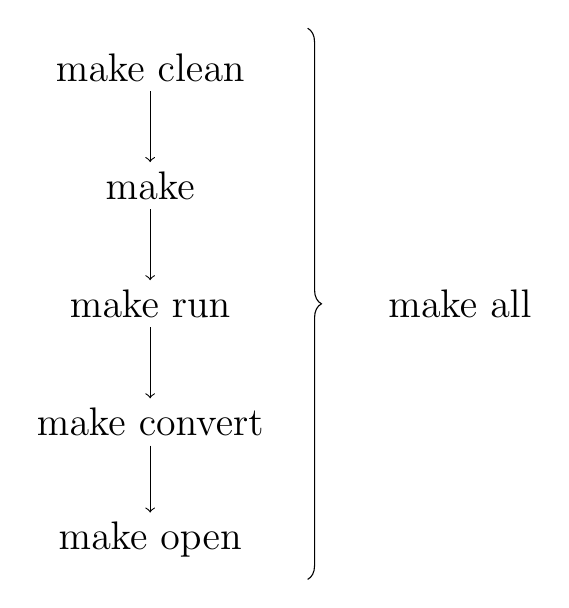
\begin{tikzpicture}[node distance=1.5cm]
      \node[](clean){\code{\Large{make clean}}};
      \node[below of=clean](make){\code{\Large{make}}};
      \node[below of=make](run){\code{\Large{make run}}};
      \node[below of=run](convert){\code{\Large{make convert}}};
      \node[below of=convert](open){\code{\Large{make open}}};
      \node[right of=run, right=1.4cm](all){\code{\Large{make all}}};
      \draw[->] (clean)--(make);
      \draw[->] (make)--(run);
      \draw[->] (run)--(convert);
      \draw[->] (convert)--(open);
      \draw[decorate,decoration={brace,amplitude=5}, right of=run, right=1.5cm]
      ($(clean)+(2.0cm,0.5cm)$)--($(open)+(2.0cm,-0.5cm)$);
    \end{tikzpicture}
  }
  \caption{Sequence of steps with the make command}
  \label{fig:appMake}
\end{figure}

\section{Self-creation of simulations}
Users can create their own simulations by writing their own programs (or by changing parameters).
If the user wishes to return the contents of the file to the default, he/she can initialize it by executing \code{make reset}, which is described in \ref{make}.
This section describes the knowledge required to create your own simulation for each file that the user edits.

\subsection{config.yml, SimulationSettings.hpp(.cpp)}
In config.yml and SimulationSettings.hpp(.cpp), define the parameters needed for the simulation. For example, the number of simulation steps, the number of
Cells, and the unit time per step of the simulation.
The description of each parameter is written as a comment in the file concerned, so please refer to them.

You can also add more parameters if necessary.
Add the simulation parameters you feel necessary to SimulationSettings.hpp, and add the code for reading from the yaml file to SimulationSettings.cpp in the try block.
These parameters are defined as static variables, so be sure to initialize them at the end of SimulationSettings.cpp.

If you want to set parameters, write the key and value in config.yaml. If you have defined your own parameters, do not forget to add them to this file as well.

*The parameters provided by default cannot be deleted.

\subsection{UserSimulation.hpp(.cpp)}
In UserSimulation.hpp(.cpp), you can define the model and initial conditions of the simulation (distribution of Cells, etc.).
Currently, the only functions that can be defined are Cell initialization (initCells), step pre-process (stepPreprocess), a mechanistic model of cell-cell interactions (calcCellCellForce), step post-process (stepEndProcess), and the calculation of cell-cell interactions ( calcCellCellForce) only.

The cell types and molecule types used in the simulation are also defined here.

Like SimulationSettings.hpp, this file also allows users to define their own variables and functions. Please add or modify functions according to the model you wish to implement.

\subsection{UserCell.hpp(.cpp)}
In UserCell.hpp(.cpp), you can define the behavior of cells.

For example, you can define when cells die, when they divide, and how their metabolism changes their energy and molecular concentrations.

The most difficult thing for users to implement is how to manage the list of existing cells.
Since MMCSS implements this tedious management in Cell.hpp(.cpp), the user only needs to implement when and under what circumstances the cells increase or decrease.
situation can be reproduced.

\subsection{UserMoleculeSpace.hpp(.cpp)}
In UserMoleculeSpace.hpp(.cpp), you can define the system of molecules you want to treat in the simulation.

The parent class, MoleculeSpace, implements several boundary conditions (Neumann, Dirichlet, and periodic boundary conditions), so no additional processing is required by the user when using these boundary conditions.

MoleculeSpace is also implemented with references to each other so that it can interact with Cell.
This feature is inherited by UserMoleculeSpace and UserCell, so users do not need to implement cumbersome class references even when simulating complex interactions between cells and molecules.

\newpage
\section{Appendix A}
\subsection{File of simulation results}
When the simulation is run, several text files with the file name cells\_step number will be output in the result directory. These files are the output of the simulation results.

The contents of the text files are separated by tab characters and contain the simulation results in the following format.

\begin{lstlisting}[caption=format of the result file]
  <Header Line>
  ID typeID X Y Z Vx Vy Vz R N_contact Contact_ID_1 Contact_ID_2 ...
\end{lstlisting}

Each of the data is described below:

\begin{itemize}
  \item ID : Identifier of Cell. A unique value is assigned.
  \item typeID : Identifier of the type of Cell. Different behaviors can be defined for each type.
  \item X : Position of X coordinate of Cell
  \item Y : Position of Y coordinate of Cell
  \item Z : Position of Z coordinate of Cell
  \item Vx : Velocity of Cell in X direction
  \item Vy : Velocity of Cell in Y direction
  \item Vz : Velocity of Cell in Z direction
  \item R : Radius of Cell
  \item N\_contact : Number of Cells in contact
  \item Contact\_ID : ID of the contacting Cell
\end{itemize}

\subsection{make commands}\label{make}
MMCSS provides several commands in addition to the make command, which is involved in running the simulation and checking the results.
The following is an explanation of these commands:

\begin{itemize}
  \item \code{make} : Build a program.
  \item \code{make run} : Run a simulation.
  \item \code{make convert} : Convert simulation result to movie file.
  \item \code{make open} : Check the simulation result movie file.
  \item \code{make clean} : Delete all object files.
  \item \code{make all} : Delete all object files, then build, run simulation, generate movie and check it all.
  \item \code{make reset} : Reset the simulation user configuration files to default.
  \item \code{make data-cleanup} : Delete all simulation products (text, images, videos).
  \item \code{make data-archive} : Zip archive the currently stored simulation results.
  \item \code{make archive-restore date=YYYYYMMDD\_HHmm} : Restore the archive contents by specifying the date and time of the archive file.
  \item \code{make archive-cleanup} : Delete all archive files.
  \item \code{make help} : Display usage and explanation of the commands registered in the Makefile.
\end{itemize}

\section{Appendix B : Samples}
\subsubsection{The Cluster Formation Model}
\begin{lstlisting}[caption=calcCellCellForce()]
Vec3 UserSimulation::calcCellCellForce(std::shared_ptr<UserCell> c) const noexcept
{
    auto aroundCells = cellList.aroundCellList(c);
    Vec3 force       = Vec3::zero();

    for (auto i : aroundCells) {
        if (cells[i]->getCellType() == CellType::WORKER) {
            force += Simulation::calcRemoteForce(c, cells[i]);
        }
    }
    force = force.normalize();

    for (auto i : aroundCells) {
        if (cells[i]->getCellType() != CellType::NONE) {
            force += Simulation::calcVolumeExclusion(c, cells[i]);
        }
    }

    return force.timesScalar(SimulationSettings::DELTA_TIME);
}
\end{lstlisting}

\subsection{The Network Formation Model}
\begin{lstlisting}[caption=UserSimulation.hpp]
  // add member variables
  std::vector<std::vector<bool>> bondMatrix;
  const double dMax   = 100.0;
  const double dMin   = 40.0;
  const double dEx    = 20.0;
  const double lambda = 20.0;
\end{lstlisting}

\begin{lstlisting}[caption=UserSimulation()]
  UserSimulation::UserSimulation(/* args */)
  {
      bondMatrix.resize(SimulationSettings::CELL_NUM, std::vector<bool>(SimulationSettings::CELL_NUM, false));
  }
\end{lstlisting}

\begin{lstlisting}[caption=stepEndProcess()]
  void UserSimulation::stepEndProcess() noexcept
  {
      for (int i = 0; i < cells.size(); i++) {
          cells[i]->clearAdhereCells();
          for (int j = 0; j < cells.size(); j++) {
              if (i == j) {
                  continue;
              }

              const Vec3 diff   = cells[i]->getPosition() - cells[j]->getPosition();
              const double dist = diff.length();
              if (dist <= dMin) {
                  bondMatrix[i][j] = true;
              }

              if (bondMatrix[i][j] && dist >= dMax) {
                  bondMatrix[i][j] = false;
              }

              if (bondMatrix[i][j]) {
                  cells[i]->adhere(*cells[j]);
              }
          }
      }
  }
\end{lstlisting}

\begin{lstlisting}[caption=calcCellCellForce()]
  Vec3 UserSimulation::calcCellCellForce(std::shared_ptr<UserCell> c) const noexcept
  {
      Vec3 force = Vec3::zero();
  
      for (auto cell : cells) {
          if (c->id == cell->id)
              continue;
  
          const Vec3 diff   = c->getPosition() - cell->getPosition();
          const double dist = diff.length();
  
          force += -diff.normalize().timesScalar(std::exp(-dist / lambda)).timesScalar(1.0);
  
          if (bondMatrix[c->id][cell->id]) {
              force += -diff.normalize().timesScalar(std::max((dist - dMin) / (dMax - dMin), 0.0)).timesScalar(30.0);
          }
  
          force += diff.normalize().timesScalar(std::max((dEx - dist) / dEx, 0.0)).timesScalar(30.0);
      }
  
      force = force.timesScalar(SimulationSettings::DELTA_TIME);
  
      return force;
  }
\end{lstlisting}

\subsubsection{The Cell Cluster Growth Model}
\begin{lstlisting}[caption=UserSimulation.hpp]
  // add member variables
  private:
  std::vector<std::vector<bool>> bondMatrix;
    const double dMax   = 150.0;
    const double dMin   = 80.0;
    const double dCont  = 20.0;
    const double lambda = 20.0;
\end{lstlisting}

\begin{lstlisting}[caption=UserSimulation()]
  UserSimulation::UserSimulation(/* args */)
  {
    bondMatrix.resize(SimulationSettings::CELL_NUM, std::vector<bool>(SimulationSettings::CELL_NUM, false));
  }
\end{lstlisting}

\begin{lstlisting}[caption=initCells()]
  void UserSimulation::initCells() noexcept
  {
    std::uniform_real_distribution<double> rand_r(0, 150);
    std::uniform_real_distribution<double> rand_theta(0, 2 * M_PI);
    for (int i = 0; i < SimulationSettings::CELL_NUM; i++) {
        double r     = rand_r(rand_gen);
        double theta = rand_theta(rand_gen);

        double x = r * std::cos(theta);
        double y = r * std::sin(theta);

        UserCell c(CellType::WORKER, x, y, 10);
        cells.push_back(std::make_shared<UserCell>(c));
    }
  }
\end{lstlisting}

\begin{lstlisting}[caption=stepPreprocess()]
  void UserSimulation::stepPreprocess() noexcept
  {
      int32_t preCellCount = cells.size();
  
      for (int i = 0; i < preCellCount; i++) {
          cells[i]->initForce();
      }
  
      for (int i = 0; i < preCellCount; i++) {
          cells[i]->clearAdhereCells();
          for (int j = 0; j < preCellCount; j++) {
              if (i == j) {
                  continue;
              }
  
              const Vec3 diff   = cells[i]->getPosition() - cells[j]->getPosition();
              const double dist = diff.length();
              if (dist <= dCont) {
                  bondMatrix[i][j] = true;
              }
  
              if (bondMatrix[i][j] && dist >= dMax) {
                  bondMatrix[i][j] = false;
              }
  
              if (bondMatrix[i][j]) {
                  cells[i]->adhere(*cells[j]);
              }
          }
      }
  }
\end{lstlisting}

\begin{lstlisting}[caption=calcCellCellForce()]
  Vec3 UserSimulation::calcCellCellForce(std::shared_ptr<UserCell> c) const noexcept
  {
      Vec3 force = Vec3::zero();
  
      for (auto cell : cells) {
          if (c->id == cell->id)
              continue;
  
          const Vec3 diff   = c->getPosition() - cell->getPosition();
          const double dist = diff.length();
  
          if (bondMatrix[c->id][cell->id]) {
              if (c->adhereCells.size() <= 3) {
                  force += diff.normalize().timesScalar((dMax - dist) / dMax).timesScalar(2.0);
              } else {
                  force += -diff.normalize().timesScalar(std::max(0.0, (dist - dMin) / (dMax - dMin))).timesScalar(2.0);
              }
          }
  
          force += -diff.normalize().timesScalar(std::exp(-dist / lambda)).timesScalar(0.05);
  
          if (dist < dCont) {
              force += diff.normalize().timesScalar((dCont - dist) / dCont).timesScalar(10.0);
          }
      }
  
      force = force.timesScalar(SimulationSettings::DELTA_TIME);
  
      return force;
  }
\end{lstlisting}

\subsubsection{The Cell Cluster Rotation Model}
\begin{lstlisting}[caption=calcCellCellForce()]
Vec3 UserSimulation::calcCellCellForce(std::shared_ptr<UserCell> c) const noexcept
{
    auto aroundCells            = cellList.aroundCellList(c);
    Vec3 force                  = Vec3::zero();
    const Vec3 center           = Vec3(0, 0, 0);
    const Vec3 diff_from_center = c->getPosition() - center;
    Vec3 force_cont             = Vec3::zero();

    constexpr double COEFFICIENT   = 1.0;
    constexpr double REPUlSION_C   = 0.20;
    constexpr double REPULSION_LEN = 15;
    constexpr double BONDING_LEN   = 5;

    force += -diff_from_center.normalize().timesScalar(COEFFICIENT);

    for (auto i : aroundCells) {
        auto cell = cells[i];

        if (c->id == cell->id)
            continue;

        const Vec3 diff   = c->getPosition() - cell->getPosition();
        const double dist = diff.length();

        if (dist < REPULSION_LEN) {
            force += diff.timesScalar(1.0 / dist).timesScalar(REPUlSION_C).timesScalar((REPULSION_LEN - dist) / REPULSION_LEN);
        }

        const Vec3 v = cell->getVelocity();
        if (dist < BONDING_LEN) {
            force_cont += v;
        }
    }

    force += force_cont.normalize().timesScalar(0.2);
    force = force.timesScalar(SimulationSettings::DELTA_TIME);

    return force;
}
\end{lstlisting}

\subsection{The Signal Molecular Diffusion Model}
\begin{lstlisting}[caption=stepEndProcess()]
void UserSimulation::stepEndProcess() noexcept
{
    for (int32_t i = 0; i < (int32_t)cells.size(); i++) {
        if (cells[i]->getCellType() == CellType::DEAD || cells[i]->getCellType() == CellType::NONE) {
            continue;
        }

        Vec3 pos = cells[i]->getPosition();
        cells[i]->updateState(moleculeSpaces[0]->getMoleculeNum(pos));
    }
}
\end{lstlisting}

\begin{lstlisting}[caption=calcCellCellForce()]
Vec3 UserSimulation::calcCellCellForce(std::shared_ptr<UserCell> c) const noexcept
{
    return Vec3::zero();
}
\end{lstlisting}

Add the following to member variables and member functions of class UserCell:

\begin{lstlisting}[caption=class UserCell(UserCell.hpp)]
    private:
    double cAMP               = 0;
    double activeReceptor     = 0.0;
    double diffCamp           = 0;
    double diffActiveReceptor = 0;
    static constexpr double C       = 10;
    static constexpr double K1      = 0.036;
    static constexpr double K2      = 0.666;
    static constexpr double L1      = 10;
    static constexpr double L2      = 0.005;
    static constexpr double Q       = 4000;
    static constexpr double SIGMA   = 6.0;
    static constexpr double Ki      = 1.7;
    static constexpr double Ke      = 5.4;
    static constexpr double Kt      = 0.9;
    static constexpr double ALPHA   = 1;
    static constexpr double H       = 5;
    static constexpr double THETA   = 0.01;
    static constexpr double LAMBDA  = 0.01;
    static constexpr double EPSILON = 1;

    public:
    double emitMolecule(int32_t moleculeId) noexcept override;
    double calcSynthesis(double extracellularCAMP) const noexcept;
    double f1(double cAMP) const noexcept;
    double f2(double cAMP) const noexcept;
    double calcInactiveReceptor(double extracellularCAMP) const noexcept;
    double calcActiveReceptor(double extracellularCAMP) const noexcept;

    void setDiffState(double extracellularCAMP) noexcept;
    void updateState(double extracellularCAMP) noexcept;
\end{lstlisting}

The added member function definitions for class UserCell are shown below:

\begin{lstlisting}[caption=class UserCell(UserCell.cpp)]
double UserCell::emitMolecule(int32_t moleculeId) noexcept
{
    return cAMP * Kt / H;
}

double UserCell::calcSynthesis(double extracellularCAMP) const noexcept
{
    const double y   = (activeReceptor * extracellularCAMP) / (1.0 + extracellularCAMP);
    const double num = ALPHA * (LAMBDA * THETA + EPSILON * y * y);
    const double den = 1 + ALPHA * THETA + EPSILON * y * y * (1 + ALPHA);
    const double phi = num / den;

    return Q * SIGMA * phi / (Ki + Kt);
}

double UserCell::f1(double cAMP) const noexcept
{
    return (K1 + K2 * cAMP) / (1 + cAMP);
}

double UserCell::f2(double cAMP) const noexcept
{
    return (K1 * L1 + K2 * L2 * C * cAMP) / (1 + C * cAMP);
}

void UserCell::setDiffState(double extracellularCAMP) noexcept
{
    diffCamp = calcSynthesis(extracellularCAMP);
    diffActiveReceptor = (-activeReceptor * f1(extracellularCAMP) + (1.0 - activeReceptor) * f2(extracellularCAMP));
}

void UserCell::updateState(double extracellularCAMP) noexcept
{
    cAMP = diffCamp;
    activeReceptor += diffActiveReceptor * SimulationSettings::DELTA_TIME;
    activeReceptor = std::max(0.0, activeReceptor);
}
\end{lstlisting}

\begin{lstlisting}[caption=class UserMoleculeSpace(UserMoleculeSpace.hpp)]
private:
    const double _D = 0.024 * 1000000.0;
\end{lstlisting}

\begin{lstlisting}[caption=calcConcentrationDiff()]
void UserMoleculeSpace::calcConcentrationDiff() noexcept
{
    constexpr double hydrolysisCoefficient = 5.4;

    for (u_int32_t x = 1; x <= width; x++) {
        for (u_int32_t y = 1; y <= height; y++) {
            for (u_int32_t z = 1; z <= depth; z++) {
                deltaMoleculeSpace[x][y][z] = diffuse(x, y, z);
                deltaMoleculeSpace[x][y][z] += -hydrolysisCoefficient * moleculeSpace[x][y][z];
            }
        }
    }

    const int32_t width  = SimulationSettings::FIELD_X_LEN;
    const int32_t height = SimulationSettings::FIELD_Y_LEN;
    const int32_t depth  = SimulationSettings::FIELD_Z_LEN;
    
    for (u_int32_t i = 0; i < cells.size(); i++) {
        std::shared_ptr<UserCell>& cell = cells[i];
            
        int32_t x = (int32_t)((cell->getPosition().x + width / 2)) + 1;
        int32_t y = (int32_t)((cell->getPosition().y + height / 2)) + 1;
        int32_t z = (int32_t)((cell->getPosition().z + depth / 2)) + 1;

        deltaMoleculeSpace[x][y][z] += cell->emitMolecule(ID);
    }

    for (u_int32_t i = 0; i < cells.size(); i++) {
        int32_t x = (int32_t)((cells[i]->getPosition().x + width / 2)) + 1;
        int32_t y = (int32_t)((cells[i]->getPosition().y + height / 2)) + 1;
        int32_t z = (int32_t)((cells[i]->getPosition().z + depth / 2)) + 1;

        cells[i]->setDiffState(moleculeSpace[x][y][z]);
    }
}
\end{lstlisting}

\begin{lstlisting}[caption=config.yaml]
cell:
  cell_seed: 10 # Seed value used to set cell location, etc.
  cell_num: 500000 # initial number of cells. It becomes very heavy when the number of cells is increased. Find out why.
  position_update_method: EULER # select from AB4, AB3, AB2, EULER

simulation:
  simulation_step: 100000 # Select from AB4, AB3, AB2, EULER
  sim_step: 100000 # Total number of simulation steps
  output_interval: 100 # Output interval
  field_x_len: 1024 # Length of the x-coordinate of the simulation field
  field_y_len: 1024 # length of the y-coordinate of the simulation field
  field_z_len: 0 # length of the simulation field in z-coordinate
  delta_time: 0.001 # time in simulation per step

molecule:
  default_molecule_nums: # initial number of each molecule (expressed as a list)
      - 3000
  delta_time: 0.001
  field_x_len: 1024 # length of x-coordinate in field for molecule management >= 1
  field_y_len: 1024 # length of y-coordinate of the molecular control field >= 1
  field_z_len: 1 # length of the z-coordinate of the molecular control field >= 1
  boundary_condition: # Boundary condition for the molecular control field
      xy1: NEUMANN
      xy2: NEUMANN
      yz1: NEUMANN
      yz2: NEUMANN
      zx1: NEUMANN
      zx2: NEUMANN

# Not used in this case, so not relevant
cell_list:
  use_cell_list: false # whether cell list is used or not
  grid_size_mag: 32 # grid division factor in cell list. Minimum must be 1 and value must be 2^n.
  search_radius: 256 # cells within this radius (difference of position) are used for force calculation.
\end{lstlisting}

\end{document}